\documentclass[11pt,a4paper,titlepage]{article}
\usepackage{graphicx}
\usepackage[margin=1in]{geometry}
%\usepackage{titling}
\usepackage[hidelinks]{hyperref}




\DeclareGraphicsExtensions{.png}
\DeclareGraphicsExtensions{.jpg}

\begin{document}
\begin{titlepage}
	\begin{center}
		
		\begin{figure}[t]
			\centering
			
\includegraphics[width=350px]{UP_Logo.png}
		\end{figure}		
	
	
	\begin{flushright} 
		
		\textbf{\LARGE COS 301 Main Project}
		\newline \newline \newline
		\textbf{\LARGE Requirements and Design Specifications}
		\newline \newline \newline
 		\textbf{\LARGE ThinkTech}
		\newline \newline \newline
	\end{flushright}
		
		\vspace{1 cm}
		
		\LARGE{\textbf{Group Members: }}
		
		%\begin{minipage}{0.4\textwidth}

		\begin{flushright} \large
			Lelethu Zazaza 13028023\newline
			Goodness Adegbenro 13046412\newline
		\end{flushright}
		%\end{minipage}
		
	
		
		\textbf{Git repository link:\\}
		 \url{ https://github.com/COS301-ThinkTech}
		
		\vfill
		
		{\LARGE Version 0.1}
		\\
		{\large \today}		
		
		
	\end{center}
\end{titlepage}


\tableofcontents
\pagebreak

\section{Vision and scope}
\subsection{Project background}
\subsection{Project vision}
\subsection{Project scope}

% Include auxillary files here:  \input{file} 


\newpage	
\section{Use case prioritization}
\subsection{Critical}
\begin{itemize}
  \item createNewFlowchart
\end{itemize}
\subsection{Important}
\begin{itemize}
  \item addFlowchartComponent
  \item editFlowchartComponent
  \item saveFlowchart
\end{itemize}
\subsection{Nice-To-Have}

\newpage
\section{Use cases}
	
\subsection{deleteFlowchartProject}
The deleteFlowchartProject use case serves the purpose of removing a flowchart project.

\subsubsection{Use case diagram}
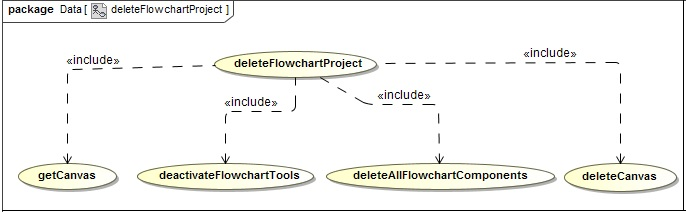
\includegraphics[width=500px]{deleteFlowchartProjectUseCase.jpg}

\subsubsection{Activity diagram}
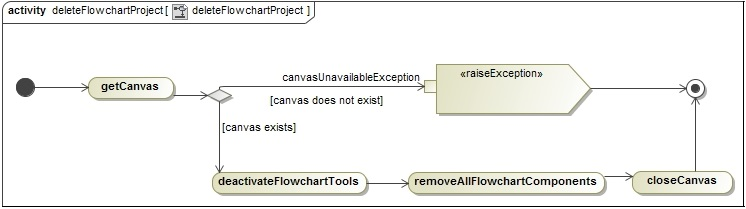
\includegraphics[width=500px]{deleteFlowchartProject.jpg}

\subsection{editFlowchartComponent}
The editFlowchartComponent use case provides functionality for the user to edit each component of the flowchart on a canvas.\newline\newline
\textbf{Pre Condition:} Component must have been added\newline\newline
\textbf{Post Condition:} Component has been edited

\subsubsection{Use case diagram}
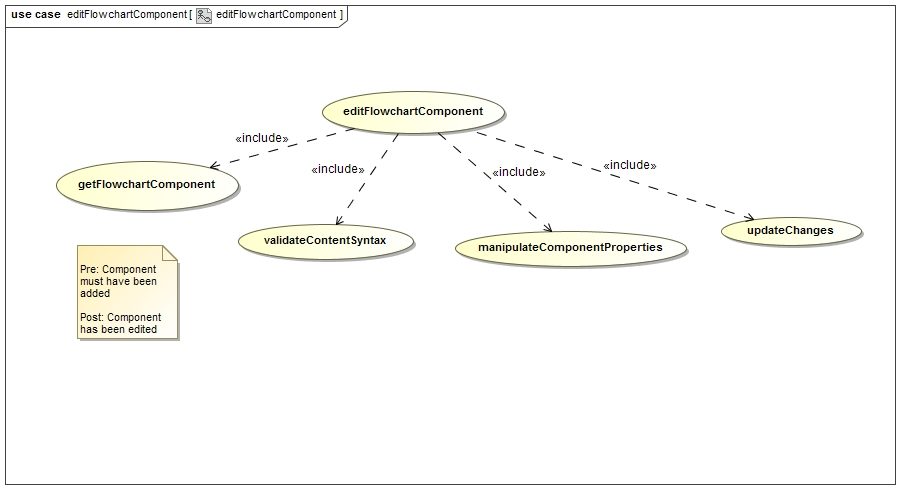
\includegraphics[width=500px]{editFlowchartComponentUseCase.jpg}

\subsubsection{Activity diagram}
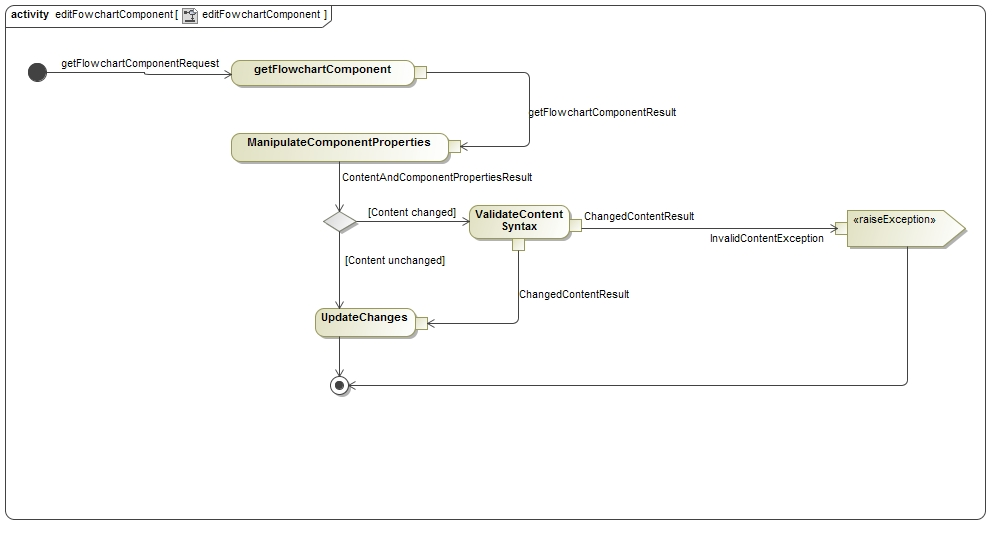
\includegraphics[width=500px]{editFowchartComponent.jpg}

\subsection{saveFlowchart}
The saveFlowchart use case provides functionality for the user to save a flowchart.\newline\newline
\textbf{Pre Condition:} Canvas is open\newline\newline
\textbf{Post Condition:} Flowchart has been saved to file

\subsubsection{Use case diagram}
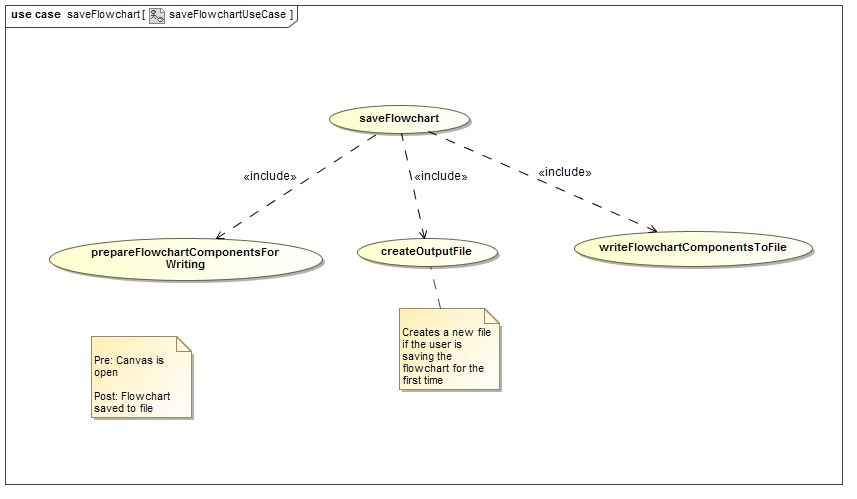
\includegraphics[width=500px]{saveFlowchartUseCase.jpg}

\subsubsection{Activity diagram}
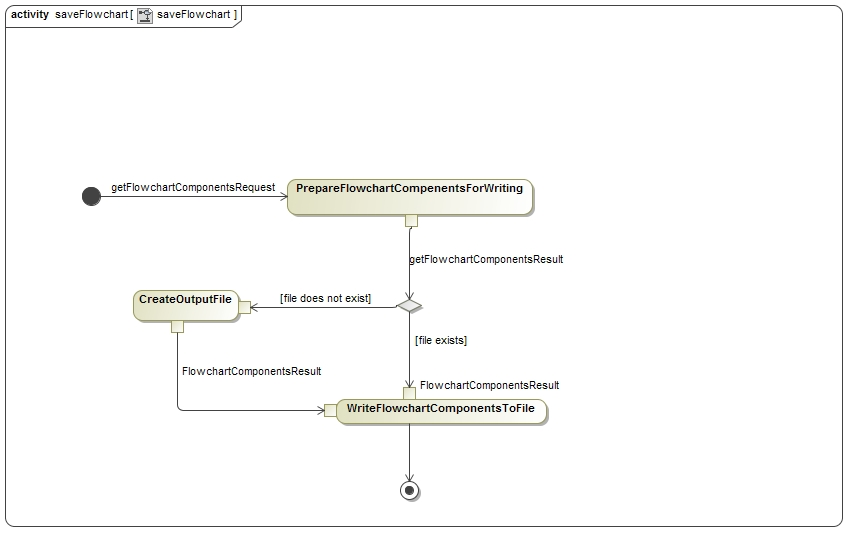
\includegraphics[width=500px]{saveFlowchart.jpg}
	
\end{document}
